\documentclass{article} % For LaTeX2e
\usepackage{nips15submit_e,times}
\usepackage{hyperref}
\usepackage{url}
\usepackage{graphicx}
%\documentstyle[nips14submit_09,times,art10]{article} % For LaTeX 2.09


\title{Hadoop Naive Bayes for 10605 15 Fall}


\author{
Jingyuan Liu\\
AndrewId: jingyual\\
\texttt{jingyual@andrew.cmu.edu} \\
}


\newcommand{\fix}{\marginpar{FIX}}
\newcommand{\new}{\marginpar{NEW}}


\nipsfinalcopy % Uncomment for camera-ready version


\begin{document}
\maketitle


\section{Question 1}


\subsection{recieve help}
I did not recieve direct help from others.

\subsection{give help}
I did not give detailed direct help to others.


\section{Question 2}
The Figure \ref{fig:wallTimeOverReducer1} shows the wall time change trend over
the number of reducers, and the time is counted from reduce 0\% to 100\%. The
Figure \ref{fig:wallTimeOverReducer2} shows the time of reducer from map 100\%
and reduce x\% to map 100\% and reducer 100\%. As we can see from the two curve,
the wall time is not reduced linearly with number of reducers.

\begin{figure}[h]
\begin{center}
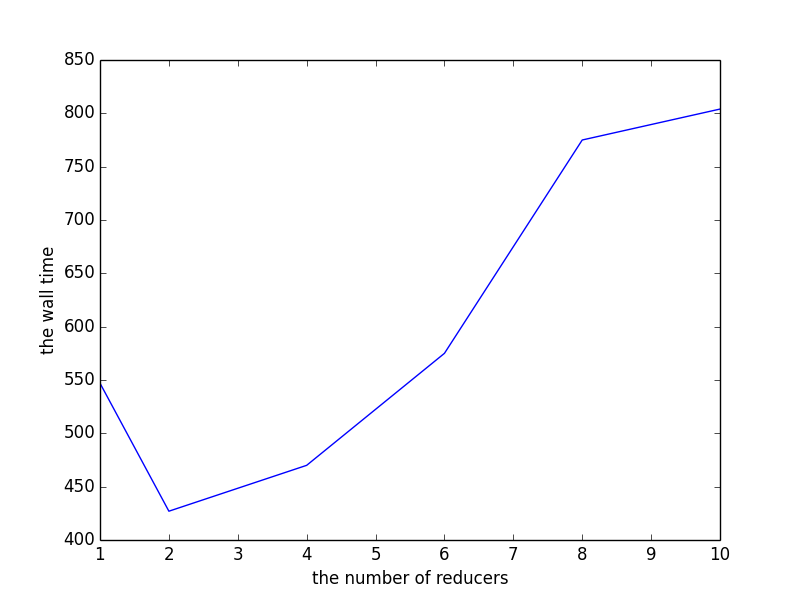
\includegraphics[width=10cm]{pic/figure_1.png}
\end{center}
\caption{The wall time over number of reducers, reducer 0\% to 100\%}
\label{fig:wallTimeOverReducer1}
\end{figure}

\begin{figure}[h]
\begin{center}
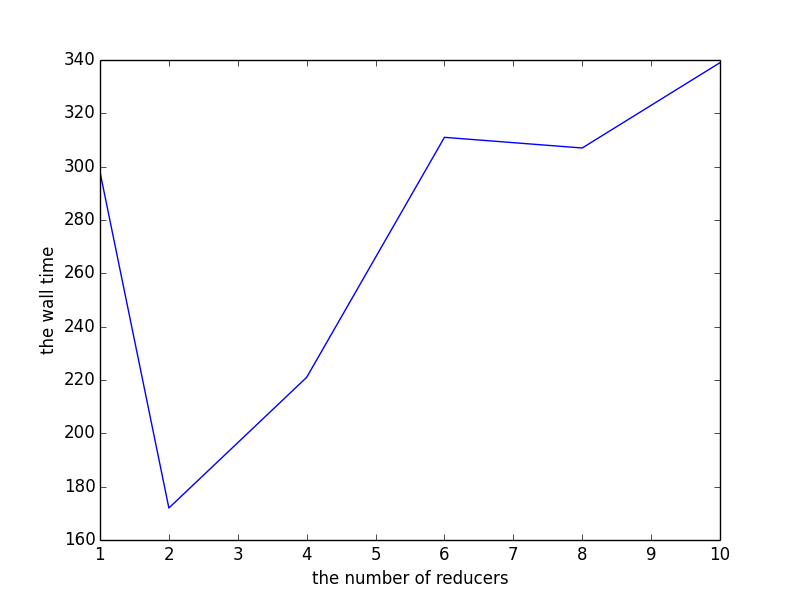
\includegraphics[width=10cm]{pic/figure_2.png}
\end{center}
\caption{The wall time over number of reducers, map 100\% and reducer x\% to
reduce 100\%}
\label{fig:wallTimeOverReducer2}
\end{figure}


Reducer contains several substeps: shuffle, sort, reduce. Shuffle step is to
transfer data, sort is to sort mapped result, and reduce is to sum results based
on mapped keys. I think several reasons may explain:

1. For shuffling step, the wall time over reducers numbers should increase with
the increase of reducers. It is because in this step, the reducers would take
more time to shuffle data to different reducers from mapper compared with less
reducers. To conclude, it would destroy disk IO for no really sane reasons and
creasily increase the network amounts of CFIF/MFIF work. (The last sentence was
referred from the apache tutorial on how to choose reducer numbers)

2. For sorting, the time complexity is o(n * log(n)), the cost time is not
linearly reduced.

3. For reduce step, the time may be not linearly. I think the cache problem
would influence the running time performances. With larger sorted datasets for a
reducer, there would be bigger cache hits rate than a smaller sorted datasets.
The cost time between cache hits and cache miss is very big, and could be very
obvious considering the dataset is large.



\section{Question 3}
I think this would adversly impact the performance of the job. Because the naive bayes
classifier mainly works on the conditional probabilities of words over labels to
decide which label would be the best label given the input words. If the
situation that most appearing word is "the" in every label and its conditionaly
probability is obviously bigger than other words, it would likely to hurt the
performances.

Let's take an example to clarify it. Suppose the score are as follows:

"W=the,Y=sport" 0.9, "W=soccer,Y=sport" 0.02, "W=statistic,Y=sport" 0.001

"W=the,Y=ML" 0.9, "W=soccer,Y=ML" 0.001, "W=statisic,Y=ML" 0.02

In these case, given a new doc with words containing "the", "soccer", the
label score of "sport" and "ML" is very close. But if we get rid of "the" word, then
we could find that "sport" label score is much bigger than "ML" label, which is
more reasonbale.

The solution is to filter those common seen "stop words". We could at first build a
word set to filter those words without specific meanings like "the", "a" and
"and" but likely to appear in many documents. We could also try to
count the number of word appearing in differnt documents, and filter those top
appearing words.



\section{Question 4}
This was for overcoming the bottleneck of program IO . As we can see, when users are
using Hadoop, they are likely to deal with large datasets. Therefore, if we use
large block size, then we can make less requests to our disks, which would be
likely to better the IO performances.

For example, suppose we are preprocessing 64Mb data. Then in HDFS, we just need
1 request, while in other normal FS, we would need 16 times 1024 requests.



\section{Question 5}
From the instance monitoring figure \ref{fig:monitoring}, we would see that the
CPU utilization is not always very high. The CPU Utilization was growing at the
first part, then kept on 100\% running for a while, and decreasing at last. The
trend was similar for Disk Write and Read Operations. However, the peak of CPU
Utilization and Disk Operations were not totally overlapped. The Disk Operations
peak came earlier.

\begin{figure}[h]
\begin{center}
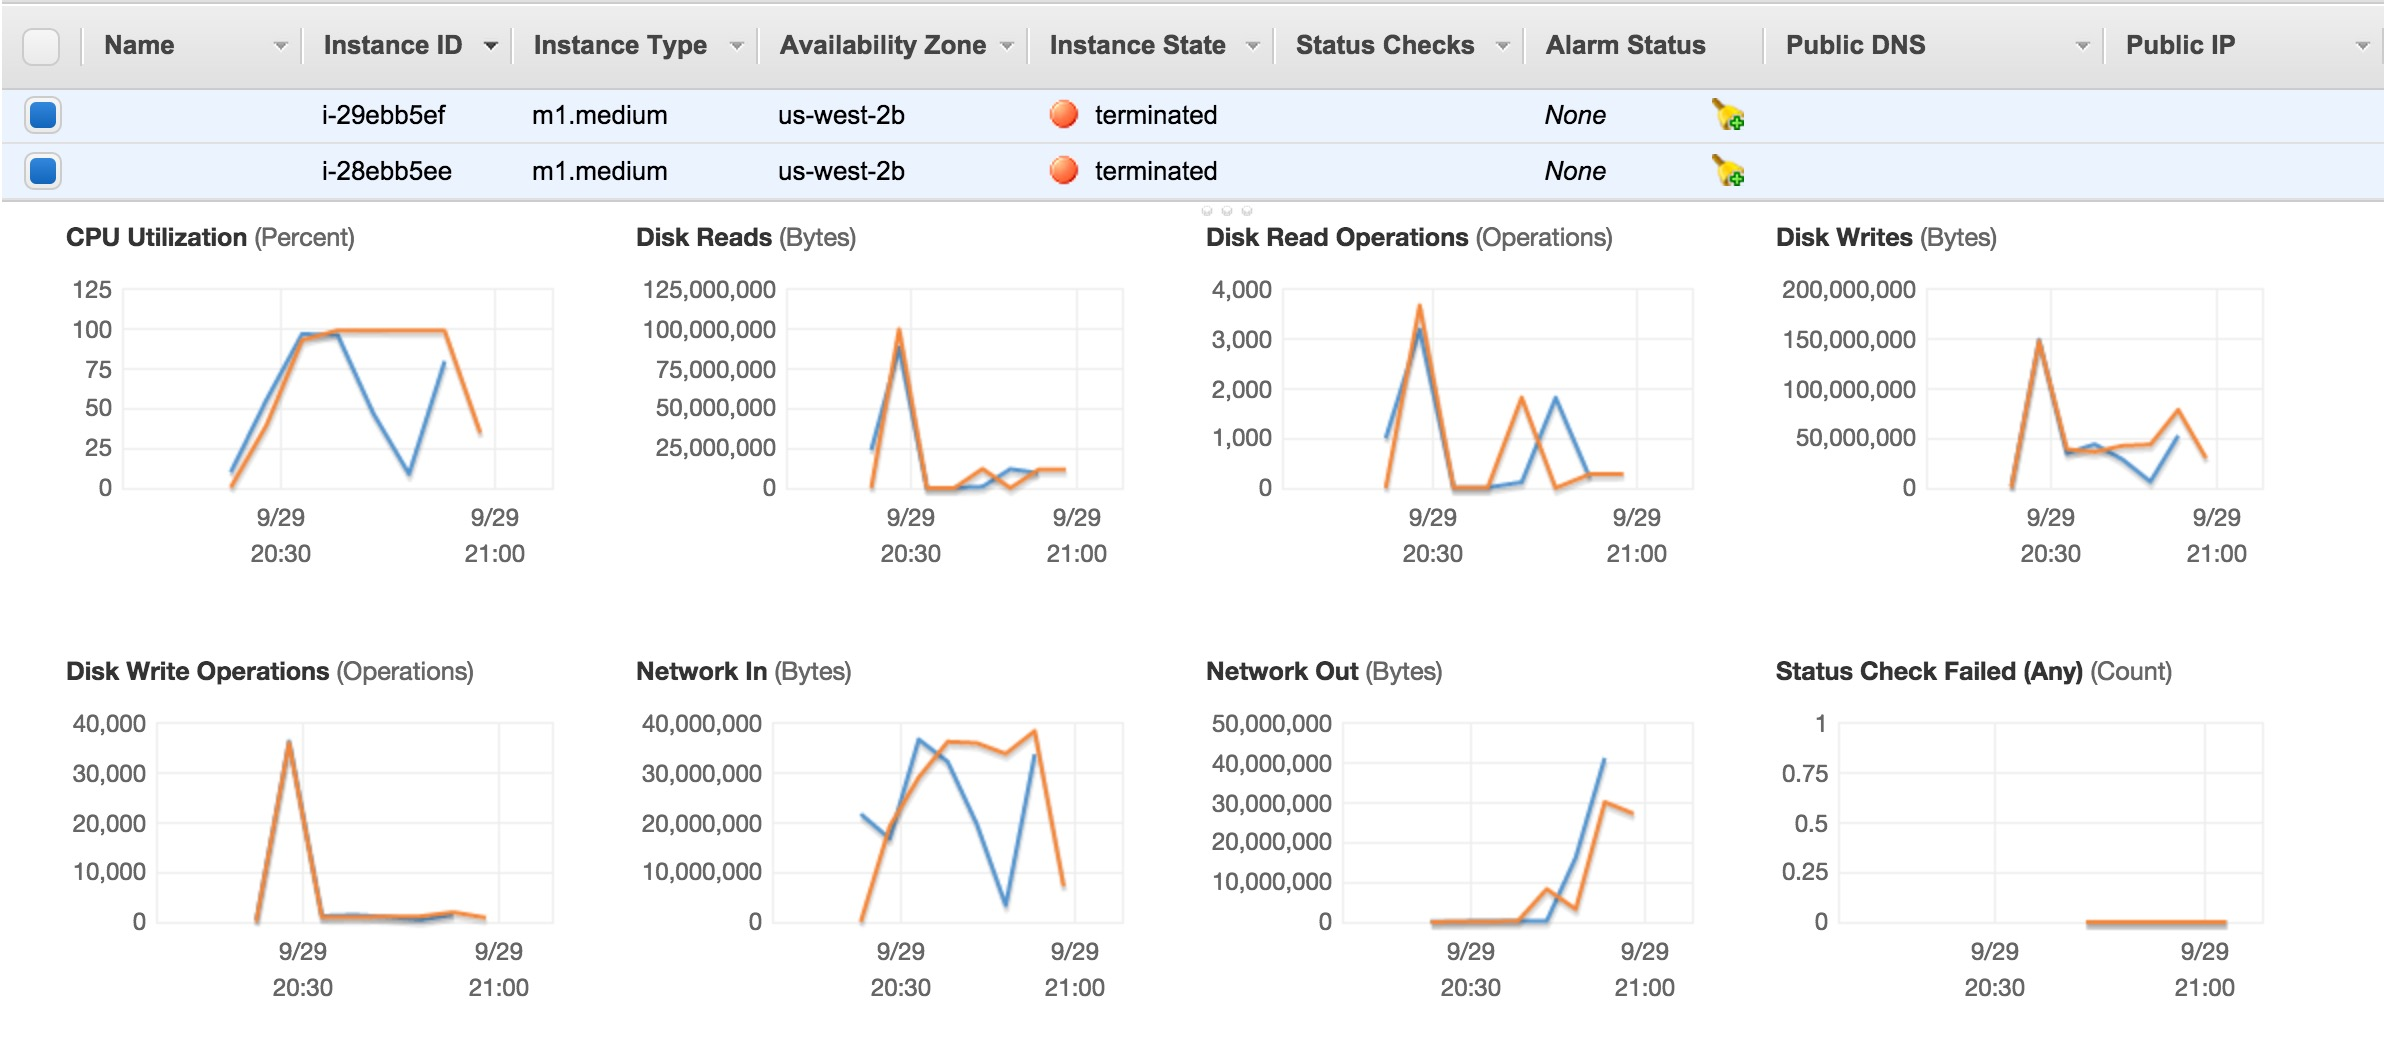
\includegraphics[width=14cm]{pic/figure_3.png}
\end{center}
\caption{Monitoring running instances}
\label{fig:monitoring}
\end{figure}

The reason why CPU Utilization would perform in this trend is the calculation
demands were different in different states of the program. We can simply define
three steps : the "mapping" step, the "sorting", and the "reduceing" step, and
the goals of each step are respectively, mapping data, sorting mapped data, and
reducing sorted data. The most CPU demanding step is obviously the sorting step,
at which the CPU Utilization reaches its peak. So we can see the trend that CPU
Utilization is increasing then decreasing.

In order to decrease the running time, we need to consider about how to decrease
the peak CPU Utilization in "sorting" step and properly increase CPU Utilization
in "mapping" or "reducing" step. A good way as mentioned in the class is to add
a combiner in the program. Without a combiner, a reducer starts after all mapper
are done and data are sorted in partition. Combiners can help us do some reducing
while waiting for some other stuffs, like sorting, and avoid moving all of that data
in the network, which are very expensive. Adding a combiner in the "mapping"
steps would increase the CPU Utilization in this part, but decrease the
overall CPU Utilization in all three steps considering that the bottleneck was
the "sorting" step.



\end{document}
